% !TEX TS-program = pdflatex
% !TEX encoding = UTF-8 Unicode

% This is a simple template for a LaTeX document using the "article" class.
% See "book", "report", "letter" for other types of document.

\documentclass[11pt]{article} % use larger type; default would be 10pt

\usepackage[utf8]{inputenc} % set input encoding (not needed with XeLaTeX)

%%% Examples of Article customizations
% These packages are optional, depending whether you want the features they provide.
% See the LaTeX Companion or other references for full information.

%%% PAGE DIMENSIONS
\usepackage{geometry} % to change the page dimensions
\geometry{a4paper} % or letterpaper (US) or a5paper or....
% \geometry{margin=2in} % for example, change the margins to 2 inches all round
% \geometry{landscape} % set up the page for landscape
%   read geometry.pdf for detailed page layout information

\usepackage{graphicx} % support the \includegraphics command and options

% \usepackage[parfill]{parskip} % Activate to begin paragraphs with an empty line rather than an indent

%%% PACKAGES
\usepackage[font=small,format=plain,labelfont=bf,up,textfont=it,up]{caption} % for nice captions
\usepackage{booktabs} % for much better looking tables
\usepackage{array} % for better arrays (eg matrices) in maths
\usepackage{paralist} % very flexible & customisable lists (eg. enumerate/itemize, etc.)
\usepackage{verbatim} % adds environment for commenting out blocks of text & for better verbatim
\usepackage{subfig} % make it possible to include more than one captioned figure/table in a single float
% These packages are all incorporated in the memoir class to one degree or another...
\usepackage[table]{xcolor} % colors for the tables


%%% HEADERS & FOOTERS
\usepackage{fancyhdr} % This should be set AFTER setting up the page geometry
\pagestyle{fancy} % options: empty , plain , fancy
\renewcommand{\headrulewidth}{0pt} % customise the layout...
\lhead{}\chead{}\rhead{}
\lfoot{}\cfoot{\thepage}\rfoot{}

%%% SECTION TITLE APPEARANCE
\usepackage{sectsty}
\allsectionsfont{\sffamily\mdseries\upshape} % (See the fntguide.pdf for font help)
% (This matches ConTeXt defaults)

%%% ToC (table of contents) APPEARANCE
\usepackage[nottoc,notlof,notlot]{tocbibind} % Put the bibliography in the ToC
\usepackage[titles,subfigure]{tocloft} % Alter the style of the Table of Contents
\renewcommand{\cftsecfont}{\rmfamily\mdseries\upshape}
\renewcommand{\cftsecpagefont}{\rmfamily\mdseries\upshape} % No bold!

%%% BIBLIOGRAPHY
\usepackage{natbib}
\usepackage{url}


%%% END Article customizations

%%% The "real" document content comes below...

\title{Automated Reasoning in AI\\
Assignment 2: Sudoku as a CSP}
\author{Armon Toubman \and Torec Luik}
%\date{} % Activate to display a given date or no date (if empty),
         % otherwise the current date is printed

\begin{document}
\maketitle

\begin{abstract}
We modeled the Sudoku game as a CSP and solved it using a search tree. The initial backtracking algorithm provides awful computation times for this particular problem. We added the general constraint propagation technique AC-3 (MAC) and specific Sudoku-solving techniques to filter the domains of our variables. The results are convincing with the latter techniques, reducing computation time on two testsets respectively from approximately 10 minutes to 10 seconds and 2 hours to 3 seconds.
\end{abstract}

\section{Introduction}
\label{sec:intro}
The popular Sudoku puzzle can be seen as a Constraint Satisfaction Problem (CSP). For this assignment, we will implement a CSP solver for solving Sudoku puzzles, including optimizations specifically for Sudokus. This will be used to find answers to our research question, which is to find an efficient solver for CSP problems. Section~\ref{sec:sudokuCSP} gives a short introduction to Sudokus as CSPs. Section~\ref{sec:search} describes the solving algorithm we used. The optimizations we used are explained in section~\ref{sec:optim}. Implementation details can be found in section~\ref{sec:impl}. Section~\ref{sec:results} provides our experimental setup and findings, while in section~\ref{sec:disc} we discuss the effectiveness of the optimizations. Finally, section~\ref{sec:concl} concludes this report.

\begin{table}[htbp]
\caption{An example Sudoku from one of our testsets.}
    \label{tab:sudoku_initial}
    \begin{center}
        \scalebox{0.75}{
        \begin{tabular}{||c|c|c||c|c|c||c|c|c||}
        \hline
        \hline
         & 9 & 4 &  &  &  & 1 & 3 & \\
        \hline
         &  &  &  &  &  &  &  & \\
        \hline
         &  &  &  & 7 & 6 &  &  & 2\\
        \hline
        \hline
         & 8 &  &  & 1 &  &  &  & \\
        \hline
         & 3 & 2 &  &  &  &  &  & \\
        \hline
         &  &  & 2 &  &  &  & 6 & \\
        \hline
        \hline
         &  &  &  & 5 &  & 4 &  & \\
        \hline
         &  &  &  &  & 8 &  &  & 7\\
        \hline
         &  & 6 & 3 &  & 4 &  &  & 8\\
        \hline
        \hline
        \end{tabular}}
    \end{center}
\end{table}


\section{Sudoku as a Constraint Satisfaction Problem}
\label{sec:sudokuCSP}

A completed (9x9) Sudoku puzzle has the numbers 1 to 9 appearing exactly once in every row, column and region. We can make the following translation from Sudoku to CSP:
\begin{itemize}
\item Variables: Not-assigned cells of a Sudoku. In other words: cells we are not sure about.
\item Assignment: Cells with assigned values.
\item Constraints: As just stated,  the numbers 1 to 9 appearing exactly once in every row, column and region.
\item Domains of the variables: At the start, the possible values of not-assigned cells are 1 to 9.
\item Consistency: An assignment is consistent if the same value does not appear more than once per row, column and region.
\item Termination: A solution is complete if there are no variables (empty cells) left. Provided the initial problem is valid, the solving process should always terminate succesfully.
\end{itemize}

\section{Search Algorithm}
\label{sec:search}

When we consider the Sudoku as a CSP with a sequence of variables, we can create a search tree for this CSP. Here the nodes of the tree are CSP's and the root is our starting CSP (i.e. the initial Sudoku). See also Figure~\ref{fig:basic_tree}. First constraint propagation is applied to the current CSP. Then, if the resulting CSP is not a leaf, one of its variables is split up. For every value in its domain, a new child will be added to the tree. This process contintues until the leaf is a correct solution (i.e. all variables are instantiated and adhere to the constraints).

\begin{figure}[htbp]
\begin{center}
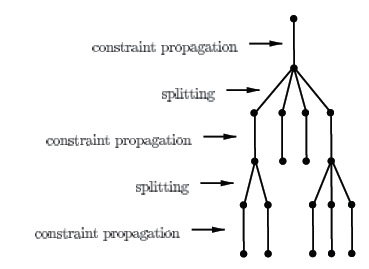
\includegraphics{tree.png}
\caption{Example of a CSP search tree. From Constraint Programming - lecture 3 (CSP) Algorithms. }
\label{fig:basic_tree}
\end{center}
\end{figure}

\subsection{The Backtracking Algorithm}
\label{sec:bt}

For creation and traversal of our Search Tree, we started with the backtracking algorithm as described in the assignment description and shown in Figure~\ref{code:BT}.

\begin{figure}
\begin{verbatim}
procedure BT(X:variables, V:assignment, C:constraints)
    if X={} then return V
    x := select a not-yet assigned variable from X
    for each value h from the domain of x do
        if consistent(V+{x/h}, C) then
            R := BT(X-{x}, V+{x/h}, C)
        if R != fail then return R
    end for
    return fail
end BT
\end{verbatim}
\caption{Basic Backtracking Algorithm}
\label{code:BT}
\end{figure}

In short, this algorithm takes a cell that is not yet assigned a value, and for each value in its domain creates a new branch in the search tree. The branches recursively create their own branches, forming a search tree. The tree is searched depth-first for a solution. The algorithm terminates if either a solution is found, or no solution exists in the search tree.

\subsection{Optimizations}
\label{sec:optim}

The Backtracking algorithm is, besides simple and effective, very inefficient. For each open cell in a Sudoku problem, the algorithm will create nine branches (one for each possible value). To solve this, we can use constraint propagation to eliminate a lot of these branches at an early stage. There are also specific Sudoku solving techniques that help rule out possible values from certain variables' domains. Pruning the search tree with these methods results in a smaller search space and therefore lower runtimes of the solver. The idea of using these techniques corresponds to constraint propagation and its application in prop labeling trees citet{Apt2003}. In this section we describe the pruning methods we used in our implementation.

\subsubsection{Constraint Propagation : Revise}
\label{sec:revise}

Our Revise method is an adjusted version of the AC-3 method as described in \citet{BartakConsistency}.
In other sources, such as \citet{Apt2003}, constraint propagation in the form of arc consistency (AC) is called MAC (Maintaining Arc Consistency).
The AC-3 method checks for arc-consistency, i.e. constraints between multiple variables. The method reduces the domain of all variables to those values that are still possible in the current solution.
It works as follows: When a value is assigned to a cell, we can rule out the assigned value as a possibility for the other cells in its row, column and region. This is because in a completed Sudoku each value should appear exactly once in each row, column and region. It is possible that this method implicitly creates a new assignment by ruling out all but one value from the domain of a cell. Because of this, the Revise method is applied until no more changes are made. This would be AC-1 in \cite{BartakConsistency}. However, after a previous revision, it is more efficient when the Revise method only checks cells that could have been affected by this revision.

\begin{table}[htbp]
\caption{First row of the Sudoku in Table~\ref{tab:sudoku_initial}. Cell 11 highlighted.}
    \label{tab:sudoku_frstrow}
    \begin{comment}
\{1, 2, 3, 4, 5, 6, 7, 8, 9\}
    {11=[1, 2, 3, 4, 5, 6, 7, 8, 9], 12=[9], 13=[4], 14=[1, 2, 3, 4, 5, 6, 7, 8, 9], 15=[1, 2, 3, 4, 5, 6, 7, 8, 9], 17=[1], 16=[1, 2, 3, 4, 5, 6, 7, 8, 9], 19=[1, 2, 3, 4, 5, 6, 7, 8, 9], 18=[3]
    \end{comment}
    \begin{center}
        \begin{tabular}{|c|c|c|c|c|c|c|c|c|}
        \hline
        %\cellcolor[gray]{0.8} & 9 & 4 &  &  &  & 1 & 3 & \\
        \cellcolor[gray]{0.7} & 9 & 4 &  &  &  & 1 & 3 & \\
        \hline
        \end{tabular}
    \end{center}
\end{table}

As an example of the working of Revise, take the first cell of the Sudoku from Table~\ref{tab:sudoku_initial}, now shown in Table~\ref{tab:sudoku_frstrow_rev}. Similar to all other empty cells, its initial domain is \{1,2,3,4,5,6,7,8,9\}.
However, the values \{1,3,4,9\} are already given in the first row, so if we apply Revise, the cell's domain will be reduced to \{2,5,6,7,8\}.
In Table~\ref{tab:sudoku_frstrow_rev}, we can see the revised domains of all cells in the first row. Keep in mind that the columns and regions are also taken into account, which is why not all the empty cells in the row have the same reduced domain.

\begin{table}[htbp]
\caption{First row of the Sudoku in Table~\ref{tab:sudoku_initial}. Domains after applying Revise.}
    \label{tab:sudoku_frstrow_rev}
    \begin{comment}
    {11=[2, 5, 6, 7, 8], 12=[9], 13=[4], 14=[5, 8], 15=[2, 8], 17=[1], 16=[2, 5], 19=[5, 6], 18=[3]
    \end{comment}
    \begin{center}
        \begin{tabular}{|c|c|c|c|c|c|c|c|c|}
        \hline
        \cellcolor[gray]{0.7}\{2, 5, 6, 7, 8\} & 9 & 4 & \{5, 8\} & \{2, 8\} & \{2, 5\} & 1 & 3 & \{5, 6\}\\
        \hline
        \end{tabular}
    \end{center}
\end{table}

This method could be capable of solving a Sudoku by itself without ever allowing the backtracking algorithm to branch, but it would require the simplest of Sudoku assignments.

\subsubsection{Constraint Propagation : Hidden Singles}
\label{sec:hsingles}
The greatest influence from our constraint propagation comes from the Sudoku-specific technique 'Hidden Singles'. We have adopted the naming of all Sudoku-specific techniques from \url{learn-sudoku.com}\footnote{\url{http://www.learn-sudoku.com/basic-techniques.html}}, but \url{Brainbashers.com}\footnote{\url{http://www.brainbashers.com/sudokuhelp.asp}} has also been used to gather information.

The technique works as follows: Given a constraint, such as the row of domains in Table~\ref{tab:sudoku_frstrow_rev}, look for any unique values. If a value is unique, such as the 7 in the first cell, we can deduce that this variable should be assigned this value for the constraint to hold.
This is one of the most powerful techniques available in solving Sudokus. A succesful application of hidden singles will provide a new given value, reducing other variables' domains. As such, when this manner of constraint propagation is applied in combination with the loop of the previously discussed Revise, most of the easier Sudokus can be solved without ever branching out into a tree.

\subsubsection{Constraint Propagation : Naked Pairs}
\label{sec:npairs}
Naked Pairs is the third constraint propagation technique we introduce in our program. Similarly to the previously discussed technique, we look for values that are only possible in certain cells. However, with naked pairs, we look for a combination of two values in a set of constrained variables (i.e. row,column,region).
Take the example in Table~\ref{tab:nakedpairs}. Cells 4 and 5 of this example contain the same pair of values. This means that these values must be in these two cells and thus they can be removed from the other variables' domains. The example then provides us a lot of new givens after applying this technique, shown in Table~\ref{tab:nakedpairs_after}.
While it is made-up, Table~\ref{tab:nakedpairs} still shows that the technique has the potential to be a powerful constraint propagater as well. We combine it together with Revise and the other constraint propagation techniques.

\begin{table}[htbp]
    \caption{Fictional row of a Sudoku. Colored cells represent a naked pair.}
    \label{tab:nakedpairs}
    \begin{center}
        \begin{tabular}{|c|c|c|c|c|c|c|c|c|}
        \hline
        \{2, 5, 7\} & 9 & 4 & \cellcolor[gray]{0.7}\{2, 5\} & \cellcolor[gray]{0.7}\{2, 5\} & \{2, 5, 6\} & 1 & 3 & \{2, 5, 8\}\\
        \hline
        \end{tabular}
    \end{center}
\end{table}

\begin{table}[htbp]
    \caption{Fictional row of a Sudoku. Corresponds to Table~\ref{tab:nakedpairs} after application of the naked pairs technique.}
    \label{tab:nakedpairs_after}
    \begin{center}
        \begin{tabular}{|c|c|c|c|c|c|c|c|c|}
        \hline
        \cellcolor[gray]{0.7}7 & 9 & 4 & \{2, 5\} & \{2, 5\} & \cellcolor[gray]{0.7} 6 & 1 & 3 & \cellcolor[gray]{0.7} 8\\
        \hline
        \end{tabular}
    \end{center}
\end{table}

\subsubsection{Constraint Propagation : Hidden Pairs}
\label{sec:hpairs}
Naked Pairs is the final constraint propagation technique we introduce in our program. This technique is similar to hidden singles, however, now we look for unique pairs of hidden values instead of singles.
Take the example in Table~\ref{tab:hiddenpairs}. Cells 1 and 9 of this example contain a pair of values (7 and 8) that are not found anywhere else. This means that these values must be in these two cells and thus their domains can be reduced to these two values. This is shown in Table~\ref{tab:hiddenpairs_after}.

\begin{table}[htbp]
    \caption{Fictional row of a Sudoku. Colored cells represent a naked pair.}
    \label{tab:hiddenpairs}
    \begin{center}
        \begin{tabular}{|c|c|c|c|c|c|c|c|c|}
        \hline
        \cellcolor[gray]{0.7}\{2, 5, 6, 7, 8\} & 9 & 4 & \{2, 5\} & \{2, 5\} & \{2, 5, 6\} & 1 & 3 & \cellcolor[gray]{0.7}\{2, 5, 6, 7, 8\}\\
        \hline
        \end{tabular}
    \end{center}
\end{table}

\begin{table}[htbp]
    \caption{Fictional row of a Sudoku. Corresponds to Table~\ref{tab:hiddenpairs} after application of the hidden pairs technique.}
    \label{tab:hiddenpairs_after}
    \begin{center}
        \begin{tabular}{|c|c|c|c|c|c|c|c|c|}
        \hline
        \cellcolor[gray]{0.7}\{7, 8\} & 9 & 4 & \{2, 5\} & \{2, 5\} & \{2, 5, 6\} & 1 & 3 & \cellcolor[gray]{0.7}\{7, 8\}\\
        \hline
        \end{tabular}
    \end{center}
\end{table}

\subsubsection{Heuristics}
\label{sec:heur}
An important part of tree search is the manner in which it is traversed. Basic strategies include Depth-First and Breadth-First, the first being implemented in the BT algorithm from Figure~\ref{code:BT}. However, these are highly inefficient when the search space grows, so we need extra functions like constraint propagation to reduce the search space. Another possibility for search space reduction is the use of heuristics.
In general, when we apply a heuristic, we rank the nodes in the tree based on the heuristic and traverse the node with the smallest value first. It is dubbed Best-First tree traversal. For the optimization of our CSP problem solver, we thought of the following heuristics:
\begin{comment}
 * Heuristics : informed guess of the next step to be taken (domain dependent)
     * I.e. combine depth-first met wat slimme breadth-first
     * f(n) = g(n) + h(n) : g(n) = depth of node n, h(n) = heuristic value ?
     * Kunnen g(n) nog wel even overslaan, hoeven we geen score systeem te hebben
     * Mogelijke opties:
     *  H1: Kies Node eerder, hoe minder kinderen het heeft
     *  H2: Kies Node eerder, hoe meer zijn values al voorkomen in de Sudoku
     *  H3: Kies Node eerder, hoe meer constrained deze is (som values in row/col/reg)
     *  H4: Diepte constrainen, bvb via g(n). Misschien zijn andere nodes eerder opgelost.
     *  H5: ... andere maten die zouden kunnen aangeven of iets dichter bij solution komt.
     *
\end{comment}
\begin{itemize}
\item Pick first the variable with the smallest domain.
\item Pick first the variable with most number of constraints.
\end{itemize}

By picking a variable with a smaller domain first, this variable should be decided upon earlier than one with a greater domain. By solving a variable, we constrain the rest of the Sudoku more and thereby can probably reduce other domains, et cetera.

The number of constraints on a variable seems similar to the size of one's domain, but a variable can be doubly constrained if it has multiple constraints telling it that one of its values is impossible. The idea is that parts of the puzzle that are more constrained are easier to solve via constraint propagation. Thus, there should be a benefit to solving variables in constrained areas first.

In the actual implementation of these heuristics, there will also be time lost on retrieving the heuristical values. Therefore, the heuristics will need to have sufficient initial benefit to create any impact on the actual CSP solver's performance. Also, instead of ordering the variables by their heuristic value, as is usually done in theory, we only keep track of the variable with the lowest score during score computation. In order to capture the best effect from heuristics, we have chosen to apply these two heuristics both separately and together.

\section{Implementation}
\label{sec:impl}

The solver was written in Java (JDK version 1.6). A prototype was written in Groovy, but the dynamic typing caused a lot of overhead: it took the Groovy prototype 2 minutes and 27 seconds to solve 10 Sudokus, while the Java rewrite solved the same Sudokus in 1 second. The fastest version of our program does include some Groovy to help with threading.

Sudokus are implemented as a HashMap mapping cellnumbers to lists of values. If the list contains only one value, that value is considered as assigned to that cell. Otherwise the cell is a variable. This map is contained in a Sudoku class together with Sudoku-specific such as consistency checks, the revise and hidden pair/hidden single/naked pair methods and many helper functions. For speed, often-needed values such as the rownumber of a certain cell and all the cells in a certain column are hardcoded into immutable arrays.

The backtracking algorithm is implemented in a seperate Solver class. This class also contains methods for applying the three heuristics, since they affect the way the algorithm branches.
We have made three runnable classes: Main, MainST and Timer. MainST executes the normal solving process. The difference between Main and MainST is that Main is multithreaded. The Timer class contains code for experiments with different options in an automated way and averaging runtimes over a certain number of runs.

Calling java with the -server argument causes our program to run about three times faster than without. The difference is in the number of the optimizations the Java interpreter performs during the compilation to native bytecode. While the server compiler is supposed to start slower and run faster than the client compiler\footnote{See \url{http://java.sun.com/products/hotspot/whitepaper.html\#server}}, with our program the only noticable difference is the faster runtime.

\section{Results}
\label{sec:results}

To compare the effectiveness of our optimizations, we performed several tests. Two sets of Sudokus were used: sudoku\_training (from Blackboard) containing 1010 Sudokus of unknown difficulty, and top95, a set containing the 95 most difficult known Sudokus\footnote{\url{http://magictour.free.fr/top95}: benchmark on Sudoku fora \url{http://www.setbb.com/sudoku/}}. All tests were performed on a desktop PC with an AMD Phenom II 720BE triple core processor running at 2.8GHz and 4GB RAM.

The first test was comparing the runtimes of combinations of Hidden Singles, Hidden Pairs and Naked Pairs together with Revise. Because of time constraints, we did not test the top95 set without optimizations. It can be expected that the runtime of the top95 set without Revise compared to with Revise would be relatively greater than the difference between running sudoku\_training with and without Revise. This is because without optimizations, the Backtracking algorithm tries to solve the Sudokus purely by branching on all possible values for variable cells. The Sudokus in the top95 set all have very few givens (17, some maybe a few more), requiring more branching and backtracking to solve than the sudoku\_training set.
Table~\ref{tab:tech_results} shows the results of tests with Revise and combinations of Hidden Singles, Hidden Pairs and Naked Pairs. Table~\ref{tab:heur_results} shows the results of tests with Revise and combinations of our heuristics. Table~\ref{tab:hs+heur_results} shows the results of tests with Revise, Hidden Singles and combinations of our heuristics. These tests were to see if the effect of the heuristics changes with the use of an extra optimization. Table~\ref{tab:alles_aan} shows our runtimes with all optimizations and heuristics enabled.

\begin{table}[hp]
\begin{center}
\begin{tabular}{c c c c c c}
\hline
 Revise & Hidden Singles & Hidden Pairs & Naked Pairs & sudoku\_training & top95 \\
\hline
 &  &  &  & 9m49s & $*$ \\ % training_norv=589.495531305
x &  &  &  & 8m56s & 1h55m25s \\ % training_rv=536.094290474, top95_rv=6924.5242909
x & x & x & x & 25s & 10s \\ % training_rv_hs_hp_np_h13=25.511620738333335, top95_rv_hs_hp_np=9.685215524666667
x & x &  &  & 29s & 47s \\ % training_rv_hs=29.234435128, top95_rv_hs=47.415598335
x & x &  & x & 23s & 21s \\ % training_rv_hs_np=23.296235251333332,, top95_rv_hs_np=20.824697618666665
x & x & x &  & 28s & 16s \\ % training_rv_hs_hp=27.667227801666666,  top95_rv_hs_hp=15.692717729
x &   & x &  & 8m9s & 26m37s \\ % training_rv_hp=489.462033154, top95_rv_hp=1596.8818117199999
x &   & x & x & 1m21s & 3m51s \\ % training_rv_hp_np=81.19639021366667, top95_rv_hp_np=230.84322473
x &  &  & x & 1m17s & 19m32s \\ % training_rv_np=76.90551903866667, top95_rv_np=1172.4098914453334
\hline
\end{tabular}
\end{center}
\caption{The runtimes of our program using two different Sudoku sets with the different optimizations enabled (indicated with an x) or disabled. The times were averaged over three runs, except the revise-only trial and the trial with no optimizations which were only performed once.\\ $*$ = not run}
\label{tab:tech_results}
\end{table}

\begin{table}[hp]
\begin{center}
\begin{tabular}{c c c c c c}
\hline
 Revise & Heuristic 1 & Heuristic 3 & sudoku\_training & top95 \\
\hline
x &  &  & 8m56s & 1h55m25s \\ % training_rv=536.094290474, top95_rv=6924.5242909
x & x &  & 1m45s & 5m37s \\ % training_rv_h1=104.71135923499999, top95_rv_h1=336.839012999
x &  & x & 2m18s & 9m11s \\ % training_rv_h3=138.14704946666666, top95_rv_h3=551.151111206
x & x & x & 1m45s & 9m9s \\ % training_rv_h13=104.98554738766667, top95_rv_h13=548.8695794
\hline
\end{tabular}
\end{center}
\caption{The runtimes of our program using two different Sudoku sets with only the revise algorithm and no, one or both heuristics enabled.  The times were averaged over three runs.}
\label{tab:heur_results}
\end{table}

\begin{table}[hp]
\begin{center}
\begin{tabular}{c c c c c c}
\hline
 Revise & Hidden Singles & Heuristic 1 & Heuristic 3 & sudoku\_training & top95 \\
\hline
x & x &  &  & 29s & 47s \\ % training_rv_hs=29.234435128, top95_rv_hs=47.415598335
x & x & x &  & 25s & 30s \\ % training_rv_hs_h1=24.783181131333333, top95_rv_hs_h1=29.532021471666667
x & x &  & x & 27s & 37s \\ % training_rv_hs_h3=26.526312118000003, top95_rv_hs_h3=37.05672543666666
x & x & x & x & 26s & 26s \\ % training_rv_hs_h13=25.561958684999997, top95_rv_hs_h13=25.992425686666667
\hline
\end{tabular}
\end{center}
\caption{The runtimes of our program using two different Sudoku sets with only the revise algorithm and the hidden singles algorithm and no, one or both heuristics enabled. The times were averaged over three runs.}
\label{tab:hs+heur_results}
\end{table}

\begin{table}[hp]
\begin{center}
\begin{tabular}{c c c c c c c c}
\hline
 Revise & H. S. & H. P. & N. P. & Heur. 1 & Heur. 3 & sudoku\_training & top95 \\
\hline
x & x & x & x & x & x & 20s & 7s \\ 
x & x & x & x & x & x & 8s $*$ & 3s $*$ \\
\hline
\end{tabular}
\end{center}
\caption{The runtimes of our program using two different Sudoku sets with all optimizations and heuristics enabled. The times were averaged over three runs. \\ $*$ = multithreaded}
\label{tab:alles_aan}
\end{table}

\section{Discussion}
\label{sec:disc}
The most interesting result is that we have brought the runtime of solving the top95 set from nearly 2 hours with only Revise to 7 seconds (3 seconds multithreaded) with all optimizations and heuristics on, as can be seen in Table~\ref{tab:tech_results} and Table~\ref{tab:alles_aan}. For the sudoku\_training set the result is still great but less dramatic: from 9 minutes to 20 seconds (8 multithreaded). The effect of Hidden Pairs on the top95 set is also remarkable, reducing the runtime from 2 hours to 30 minutes.
It is also good to see that our heuristics are doing well. Even without optimizations (apart from Revise) both Heuristic 1 and 3 reduce the solving time significantly.
Finally, because the optimizations and heuristics manage to reduce the solving times a great deal on their own, it is almost surprising that the lowest runtime was achieved by activating all options. This means that all parts have some effect, even when combined.

\section{Conclusion}
\label{sec:concl}
We have written a Sudoku solver that treats Sudoku puzzles as CSPs and increased its performance by applying established CSP and Sudoku solving techniques. Our custom heuristics also have a significant effect on the performance. The lowest runtimes were achieved by combining all optimizations and heuristics.



\bibliographystyle{plainnat}
\bibliography{ref}

\end{document}
